\documentclass[11pt,a4paper]{article}
\usepackage[T1]{fontenc}
\usepackage{lmodern,microtype,amsmath,amssymb,amsthm,mathtools,booktabs,array,xcolor}
\usepackage[margin=26mm,top=24mm,bottom=24mm,headheight=15pt]{geometry}
\usepackage{fancyhdr,titlesec,pgfplots,listings}
\lstset{language=Python,basicstyle=\ttfamily\footnotesize,columns=fullflexible,keepspaces=true,showstringspaces=false,breaklines=true}
\pgfplotsset{compat=1.17}
\definecolor{ink}{HTML}{173B47}\definecolor{accent}{HTML}{176C70}\definecolor{gold}{HTML}{A4572B}
\usepackage[colorlinks=true,linkcolor=ink,citecolor=accent,urlcolor=accent]{hyperref}
\usepackage{bookmark}
\titleformat{\section}{\large\sffamily\bfseries\color{ink}}{\thesection}{.5em}{}
\titleformat{\subsection}{\normalsize\sffamily\bfseries\color{ink}}{\thesubsection}{.5em}{}
\newtheorem{theorem}{Theorem}[section]\newtheorem{lemma}[theorem]{Lemma}\newtheorem{proposition}[theorem]{Proposition}\newtheorem{corollary}[theorem]{Corollary}
\numberwithin{equation}{section}
\newcommand{\R}{\mathbb R}\newcommand{\E}{\mathbb E}\newcommand{\norm}[1]{\left\lVert #1\right\rVert}
\newcommand{\B}{\mathrm B}\newcommand{\supp}{\operatorname{supp}}\newcommand{\vol}{\operatorname{vol}}
\pagestyle{fancy}\fancyhf{}\lhead{\small\sffamily The continuous radial Tur\'an problem}\rhead{\small\sffamily Sharp constants and stability}\cfoot{\small\thepage}
\renewcommand{\headrulewidth}{.3pt}\setlength{\emergencystretch}{1.5em}\raggedbottom
\hypersetup{pdftitle={The continuous Turan problem for l1-radial functions},pdfsubject={An exact extremizer, quantitative stability, and sums of Euclidean norms}}
\begin{document}
\begin{center}
{\LARGE\bfseries\color{ink} The continuous Tur\'an problem for\\[3pt] $\boldsymbol{\ell_1}$-radial functions\par}
\vspace{5pt}{\large An exact extremizer, stability, and sums of Euclidean norms}\par\vspace{7pt}
{\small Research manuscript prepared for Keio \enspace$\cdot$\enspace 20 November 2026}
\end{center}
\begin{abstract}
Among continuous positive definite functions $f(x)=\varphi(\|x\|_1)$ on $\mathbb R^d$, normalized by $f(0)=1$ and supported in the cross-polytope of radius $R$, we prove that the largest integral is $R^d/(2^{d-1}d!)$. This determines the continuous extremal problem studied by Berdysheva and Berens and proves their conjectured separation from the unrestricted problem in every $d\ge2$. The unique extremizer is a beta average of the normalized Euclidean ball covariogram. If the integral is a fraction $1-\delta$ of the optimum, its uniform distance from the extremizer is at most $2\sqrt\delta$, and the exponent is optimal. We derive these conclusions from a correspondence that preserves the support radius, including a local inversion excluding cancellations in signed profiles. The same argument gives exact sharp constants for sums of Euclidean block norms and an explicit solution for a family of quadratic weights. Two independent appendices answer a question of Galvin on tree log-concavity and conjectures of Sun on central binomial and Catalan numbers.
\end{abstract}
\noindent\textsf{Companion results.}\enspace Appendix~\ref{sec:galvinbulk} (p.~\pageref{sec:galvinbulk}) gives trees of maximum degree $70$ with a log-concavity failure at $k\le79\alpha/80$. Appendix~\ref{sec:sun} (p.~\pageref{sec:sun}) proves Sun's two divisor-sum assertions and verifies the exact exceptional indices in OEIS A248125.
\section{The original problem}
For $R>0$ let $B_p^d(R)=\{x\in\mathbb R^d:\|x\|_p\le R\}$. A continuous function $f$ is positive definite if $\sum_{j,k} c_j\overline{c_k}f(x_j-x_k)\ge0$ for every finite choice of points and complex coefficients. Berdysheva and Berens studied the extremal integral for functions supported in $B_1^d(R)$ and depending only on $\|x\|_1$, first in the plane and then in arbitrary dimension~\cite{BB05,BB09}. Their 2016 formulation fixes $R=\pi$ and asks for the supremum of $2\int_0^\pi r^{d-1}\varphi(r)\,dr$ over their original class $\mathcal K_\pi^{(d)}$~\cite[Sec.~3, Problem~1, eq.~(4)]{BB16}. This is the continuous problem. Their discrete problem uses a different admissible class and a separate constant~\cite{BB14}.

\begin{theorem}\label{thm:original}
For $d\ge1$ and $R>0$, every continuous positive definite $f(x)=\varphi(\|x\|_1)$ supported in $B_1^d(R)$ with $f(0)=1$ satisfies
\begin{equation}\label{eq:original}
 \int_{\mathbb R^d}f(x)\,dx\ \le\ \frac{R^d}{2^{d-1}d!},\qquad
 2\int_0^R r^{d-1}\varphi(r)\,dr\ \le\ \frac{R^d}{d\,4^{d-1}} .
\end{equation}
Equality is attained by a unique profile. In particular $\kappa_\pi^{(d)}=\pi^d/(d\,4^{d-1})$ in the notation of the original problem.
\end{theorem}
The two integrals in \eqref{eq:original} differ by the shell factor $2^{d-1}/(d-1)!$. For the unrestricted problem the normalized autocorrelation of $\mathbf1_{B_1^d(R/2)}$ has integral $R^d/d!$. Hence its optimum is at least $2^{d-1}$ times the radial optimum. This proves the strict inequality conjectured just after (4) in~\cite{BB16} for every $d\ge2$. The unrestricted optimum itself is a separate question.

Previously the $2d$-monotone subclass had the exact profile $(1-r/R)_+^{2d-1}$ and the half-line value $2R^d\B(d,2d)$~\cite[Theorem~1]{BB16}. The ratio of \eqref{eq:original}'s half-line value to this lower bound is $\binom{3d-1}{d}/(2\cdot4^{d-1})$. It equals one for $d=1$ and strictly increases, since its consecutive ratio is $3(3d+1)(3d+2)/(8(d+1)(2d+1))>1$. The new optimizer therefore lies outside that subclass as soon as $d\ge2$.

\paragraph{The auxiliary question.} Which information about support survives averaging a spherical profile over random dilations? An exact recovery statement on exterior intervals will exclude cancellations of an arbitrary signed profile. A second identity reconstructs the full Fourier transform of a function from a single radial frequency parameter. Together they carry the original optimization, including the equality condition, to the Euclidean ball. Corpus entry~027 gives the Euclidean overlap profile in beta coordinates. Entry~029 treats recovery from integral mixtures and Fourier observations~\cite{VMRC}. The transfer and bounds below are proved directly.


\section{Recovering a compactly supported profile from its beta average}
Let $b\ge1$ and $n_1,\ldots,n_b\ge1$ be integers, put $D=\sum_j n_j$, and write $x=(x_1,\ldots,x_b)$ with $x_j\in\mathbb R^{n_j}$. Define
\[
 \rho(x)=\sum_{j=1}^b |x_j|_2,\quad K_R=\{x:\rho(x)\le R\},\quad
 \alpha_j=(n_j+1)/2,\quad A=\sum_j\alpha_j=(D+b)/2.
\]
Let $\mathcal P_2(R)$ and $\mathcal P_\rho(R)$ be the cones of continuous positive definite, respectively Euclidean-radial and $\rho$-radial, functions supported in their closed radius-$R$ balls in $\R^D$. The profiles are real because positive definite functions are Hermitian and these norms are even. Put $U\sim\mathrm{Beta}(1/2,(b-1)/2)$ for $b\ge2$, and $U=1$ for $b=1$. Write $G_0(s)$ for the profile of $G\in\mathcal P_2(R)$.

\begin{theorem}[Transfer at a prescribed support radius]\label{thm:transfer}
The map $G\mapsto (\mathcal L G)(x)=\E G_0(\rho(x)/\sqrt U)$ is a linear bijection $\mathcal P_2(R)\to\mathcal P_\rho(R)$. It preserves the value at zero. Its effect on mass is
\begin{equation}\label{eq:mass}
 \int \mathcal LG=M^{-1}\int G,\qquad
 M=\frac{\Gamma(A)}{\Gamma(b/2)}\prod_{j=1}^b\frac{\Gamma(1/2)}{\Gamma(\alpha_j)} .
\end{equation}
For any bounded continuous signed profile $k$, its beta average vanishes on $(R,\infty)$ if and only if $k$ vanishes on $(R,\infty)$.
\end{theorem}
For one-dimensional blocks the stochastic parametrization on unrestricted supports and the Dirichlet identity used below go back to Cambanis, Keener and Simons~\cite[Prop.~3.1, Thm.~3.1]{CKS}. The divided-difference form of the $\ell_1$-radial Fourier transform is due to Berens and Xu~\cite[Theorem~A and references]{BB16}. We give the proof for general blocks, keeping both support and normalization explicit.

\subsection{A Fourier transform determined by one line}
Use $\widehat f(\xi)=\int f(x)e^{-ix\cdot\xi}\,dx$. Fix unit vectors $e_j\in\mathbb R^{n_j}$, let $F=\widehat f$, and write $H(s)=F(se_1,\ldots,se_b)$. If $f$ is continuous, compactly supported, and $\rho$-radial, then
\begin{equation}\label{eq:diagonal}
 F(\xi)=\E H\!\left(\sqrt{\sum_j T_j|\xi_j|_2^2}\right),\qquad
 T\sim\operatorname{Dirichlet}(\alpha_1,\ldots,\alpha_b).
\end{equation}
For $b=1$ the law puts unit mass at $T_1=1$. To prove the identity, first take $f_a(x)=e^{-a\rho(x)}$, $a>0$. In $n$ dimensions the Fourier transform of $e^{-a|x|_2}$ is $c_n a(a^2+|\xi|_2^2)^{-(n+1)/2}$ for a positive constant $c_n$. This follows by inserting
\[
 e^{-ar}=\frac{a}{2\sqrt\pi}\int_0^\infty t^{-3/2}e^{-a^2/(4t)}e^{-tr^2}\,dt
\]
and Fourier transforming the Gaussian. The product of the block transforms has diagonal value proportional to $(a^2+s^2)^{-A}$. For $v_j>0$ the gamma integral, with $y_j=t T_j$ on the positive orthant, gives
\[
 \E\left(\sum_j T_j v_j\right)^{-A}=\prod_j v_j^{-\alpha_j} .
\]
Putting $v_j=a^2+|\xi_j|_2^2$ proves \eqref{eq:diagonal} for $f_a$. For compactly supported $f(x)=\varphi(\rho(x))$, the function $v\mapsto\varphi(-\log v)/v$ extends continuously by zero at $v=0$. Polynomial approximation on $[0,1]$ approximates $\varphi(r)$ by linear combinations of $e^{-ar}$ with error at most $\varepsilon e^{-r}$. This gives $L^1(\R^D)$ convergence and hence uniform convergence of both sides of \eqref{eq:diagonal}.

\subsection{The inverse map and the support estimate}
If $f\in\mathcal P_\rho(R)$, Bochner's theorem and Fourier inversion in distributions give $F\ge0$ and $\int F=(2\pi)^D f(0)$. Indeed, its finite representing measure has continuous density $(2\pi)^{-D}F$. Tonelli and coordinate dilation in \eqref{eq:diagonal} give
\begin{equation}\label{eq:moment}
 \int F=\E\prod_j T_j^{-n_j/2}\int_{\R^D} H(|\xi|_2)\,d\xi
       = M\int_{\R^D} H(|\xi|_2)\,d\xi .
\end{equation}
The Dirichlet moment is finite because $\alpha_j-n_j/2=1/2$. Let $G$ be the inverse Fourier transform of the integrable nonnegative function $M H(|\xi|_2)$. It is continuous, positive definite and radial, and $G(0)=f(0)$.

To recover its support, $H(s)=\int f(x)e^{-is\sum_j x_j\cdot e_j}\,dx$ is even and entire, and $|H(s)|\le\|f\|_1e^{R|\operatorname{Im}s|}$ since $|\sum x_j\cdot e_j|\le\rho(x)$. The even power series extends $H(\sqrt{z\cdot z})$ to an entire function of $z\in\mathbb C^D$, where $z\cdot z=\sum_{i=1}^D z_i^2$. For $z=a+ic$ any square root $w$ of $z\cdot z$ satisfies
\[
 |\operatorname{Im}w|^2=(|z\cdot z|-|a|^2+|c|^2)/2\le |c|^2.
\]
The Paley--Wiener--Schwartz theorem for a closed Euclidean ball now yields $\supp G\subset B_2^D(R)$~\cite[Thm.~7.3.1]{Hormander}. In particular $\int G=M H(0)=M\int f$.

\subsection{The forward map and its radial variable}
For $G\in\mathcal P_2(R)$ form the positive average
\begin{equation}\label{eq:physical}
 (JG)(x)=M^{-1}\E\!\left[\prod_j T_j^{-n_j/2}\ G(x_1/\sqrt{T_1},\ldots,x_b/\sqrt{T_b})\right].
\end{equation}
Dominated convergence gives continuity, and linear substitutions and positive averaging preserve positive definiteness. Cauchy--Schwarz gives $\rho(x)^2\le\sum |x_j|_2^2/T_j$. Thus $JG$ is supported in $K_R$. Its value at zero is $G(0)$. Absolute Fubini gives both $\int JG=M^{-1}\int G$ and
\begin{equation}\label{eq:forward}
 \widehat {JG}(\xi)=M^{-1}\E\widehat G(\sqrt{T_1}\xi_1,\ldots,\sqrt{T_b}\xi_b).
\end{equation}
On the distinguished line in \eqref{eq:diagonal} this is $M^{-1}\widehat G(|s|e)$ for any Euclidean unit vector $e$. For the $G$ constructed above, \eqref{eq:diagonal} restores $F$ at every frequency.

To identify the physical profile, tilt the law of $T$ by $M^{-1}\prod T_j^{-n_j/2}$. The resulting vector $W$ has Dirichlet parameters $(1/2,\ldots,1/2)$. For any $r_j\ge0$,
\begin{equation}\label{eq:cks}
 \sum_j r_j^2/W_j\ \overset{\mathrm{law}}=\ \left(\sum_jr_j\right)^2/U .
\end{equation}
Here is a direct proof of the identity~\cite[Prop.~3.1]{CKS}. For $a>0$ integrate $\prod y_j^{-1/2}e^{-a\sum r_j^2/y_j}$ over the simplex $y_j>0$, $\sum y_j=t$, using the first $b-1$ coordinates. The Laplace transform in $t$ equals
\[
 \prod_j\int_0^\infty y^{-1/2}e^{-s y-a r_j^2/y}\,dy
     =(\pi/s)^{b/2}e^{-2\sqrt{sa}\sum_jr_j}.
\]
It depends only on $\sum r_j$. Uniqueness of the Laplace transform identifies the simplex integral with its value for $(\sum r_j,0,\ldots,0)$. Equality holds at each $t>0$ by continuity, which follows by scaling to $t=1$ and dominated convergence on compact $t$-intervals. At $t=1$, normalize the measure and vary $a$ to obtain \eqref{eq:cks}, since $W_1$ has the law of $U$. The case $b=1$ is immediate. With $r_j=|x_j|_2$, \eqref{eq:physical} is precisely $JG=\mathcal LG$. Invertibility follows from \eqref{eq:forward} on the line and \eqref{eq:diagonal} on the whole frequency space.

\subsection{Exterior cancellation for signed profiles}
For $b\ge2$ write $\beta=(b-1)/2$, let $k$ be bounded and continuous, and set $\varphi(r)=\E k(r/\sqrt U)$. Substituting $v=tU$ into the beta integral gives
\begin{equation}
 \B(1/2,\beta)t^{\beta-1/2}\varphi(1/\sqrt t)
   =\int_0^t(t-v)^{\beta-1}h(v)\,dv,\qquad h(v)=v^{-1/2}k(1/\sqrt v).
\end{equation}
Here $h\in L^1(0,a)$ for every finite $a$. Let $I^\gamma h$ denote convolution on the half-line with $v^{\gamma-1}/\Gamma(\gamma)$, and put $I^0h=h$. Beta integration gives $I^\eta I^\gamma=I^{\eta+\gamma}$ for positive orders. If $\varphi=0$ on $(R,\infty)$, then $I^\beta h=0$ on $(0,R^{-2})$. Applying $I^{m-\beta}$ on that same interval for $m=\lceil\beta\rceil$ gives $I^m h=0$. Taking the $m$th distributional derivative gives $h=0$ there, and continuity gives $k=0$ on $(R,\infty)$. The reverse implication follows from $U\le1$. Taking differences proves that the beta average even determines a signed profile on each exterior interval from its values on that interval. This completes the proof of Theorem~\ref{thm:transfer}.


\section{The sharp constant and the exact profile}
Let $V=|B_2^D(R/2)|$ and $v_\rho=|K_1|$. The Euclidean ball theorem of Gorbachev and of Kolountzakis and R\'ev\'esz~\cite{KR} gives the maximal integral $V$ over $G\in\mathcal P_2(R)$, $G(0)=1$. The normalized ball autocorrelation $G_*(x)=|B_2^D(R/2)\cap(x+B_2^D(R/2))|/V$ attains it. The half-ball representation in the next section also gives a proof of this bound by Cauchy--Schwarz.

\begin{corollary}\label{cor:block}
The sharp integral $T$ in the normalized class $\mathcal P_\rho(R)$ and the value of an extremizer $f_*(x)=\varphi_*(\rho(x))$ are given by
\begin{align}
 T&=V/M=|K_{R/2}|\frac{\Gamma((D+1)/2)\Gamma(b/2)}{\sqrt\pi\,\Gamma((D+b)/2)},\label{eq:sharp-block}\\
 \varphi_*(r)&=\E H_D\left(\frac{r}{R\sqrt U}\right),\qquad
 H_D(s)=\frac{2\omega_{D-1}}{\omega_D}\int_s^1(1-t^2)^{(D-1)/2}\,dt\quad(0\le s\le1),\label{eq:hat}
\end{align}
where $\omega_j=\pi^{j/2}/\Gamma(1+j/2)$, $\omega_0=1$, and $H_D(s)=0$ for $s\ge1$.
\end{corollary}
\begin{proof}
Theorem~\ref{thm:transfer} carries the mass and the extremizer across. Slicing the two spherical caps of the Euclidean intersection gives $G_*(x)=H_D(|x|_2/R)$. To express $T$ relative to half the support body, integrate any transferred profile in shells. For any such pair the mass ratio is $(v_\rho/\omega_D)\E U^{D/2}$. Thus $T=|K_{R/2}|\E U^{D/2}$. The beta moment gives \eqref{eq:sharp-block}, including $b=1$ by continuity or the degenerate law. For $b=D=d$ the duplication formula gives $\E U^{d/2}=2^{1-d}$, and $|K_{R/2}|=R^d/d!$. This proves \eqref{eq:original}, with uniqueness established in Theorem~\ref{thm:sharp-stability}.
\end{proof}
At fixed total dimension and block count the fraction of the half-body volume in \eqref{eq:sharp-block} is independent of the individual block sizes. It is strictly smaller than one for $b\ge2$, since $0<U<1$ almost surely. The half-body autocorrelation for the unrestricted class therefore gives a strict gap for all such block norms.

\subsection{The extremizer at the center and boundary}
Write $s=r/R$, $a_D=2\omega_{D-1}/\omega_D$, $\beta=(b-1)/2$, $\nu=(D-1)/2$ and $p=\nu+1$. For $b\ge2$, $v=\sqrt U$ has density $2(1-v^2)^{\beta-1}/\B(1/2,\beta)$. Formula~\eqref{eq:hat} therefore gives the following two different endpoint laws:
\begin{align}
 1-\varphi_*(Rs)&=\frac{2a_D}{\B(1/2,\beta)}s\log(1/s)+O(s) \quad(s\downarrow0),\label{eq:cusp}\\
 \varphi_*(Rs)&\sim \frac{a_D 2^{\nu+\beta}\B(p+1,\beta)}{p\B(1/2,\beta)}(1-s)^{(D+b)/2}\quad(s\uparrow1).
 \label{eq:edge}
\end{align}
Indeed, minus the derivative with respect to $s$ is
\[
 \frac{2a_D}{\B(1/2,\beta)}\int_s^1 (1-s^2/v^2)^\nu(1-v^2)^{\beta-1}\,\frac{dv}{v} .
\]
For $s<1/4$ this integral equals $\log(1/s)+O(1)$. On $[s,1/2]$ the second factor is $1+O(v^2)$, and replacing the first by one costs at most $\int_0^1[1-(1-u^2)^\nu]du/u<\infty$ after $u=s/v$. The rest is bounded by integrability at $v=1$. Integration proves \eqref{eq:cusp}. Near $1$, $H_D(z)\sim (a_D2^\nu/p)(1-z)^p$. Substitution $v=s+(1-s)t$ in the beta average gives \eqref{eq:edge} by dominated convergence against $t^p(1-t)^{\beta-1}\,dt$. In particular the optimizer has an infinite one-sided slope at the origin for every $b\ge2$.

\paragraph{An elementary extremizer in three dimensions.} For $b=D=3$, $\sqrt U$ is uniform on $[0,1]$ and $H_3(t)=1-3t/2+t^3/2$ on its support. Direct integration gives
\begin{equation}\label{eq:three}
 \varphi_*(Rs)=1-\tfrac34s+\tfrac32s\log s-\tfrac14s^3\quad (0<s\le1),\qquad \varphi_*(0)=1.
\end{equation}
The sharp full-space mass is $R^3/24$. Substitution into the original half-line objective gives $2R^3\int_0^1s^2\varphi_*(Rs)\,ds=R^3/48$.
\begin{figure}[ht]
\centering
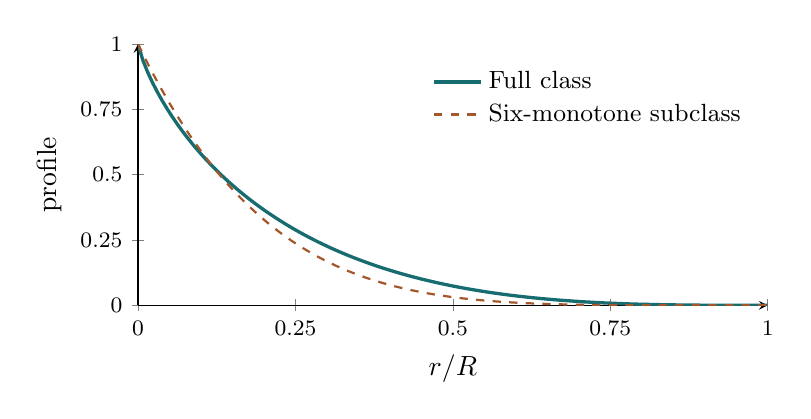
\begin{tikzpicture}
\begin{axis}[width=.79\linewidth,height=4.9cm,xmin=0,xmax=1,ymin=0,ymax=1,axis lines=left,xtick={0,.25,.5,.75,1},ytick={0,.25,.5,.75,1},tick label style={font=\footnotesize},xlabel={$r/R$},ylabel={profile},legend style={draw=none,font=\small,at={(.98,.94)},anchor=north east},legend cell align=left]
\addplot[accent,very thick,domain=.0001:1,samples=130] {1-.75*x+1.5*x*ln(x)-.25*x^3};\addlegendentry{Full class}
\addplot[gold,thick,dashed,domain=0:1,samples=100] {(1-x)^5};\addlegendentry{Six-monotone subclass}
\end{axis}\end{tikzpicture}
\caption{Exact normalized profiles in dimension three. The full extremizer initially falls faster at the origin and has the larger $r^2$-weighted integral.}
\end{figure}


\section{Uniqueness and the stability exponent}
\label{sec:sharp-stability}
Let $D$ be the ambient dimension, $b$ the number of Euclidean blocks,
$B=B_2(R/2)\subset\mathbb R^D$, and $V=|B|$. Write $T$ for the sharp
integral in the block-radial problem with $f(0)=1$. For its normalized
transfer $f=\mathcal L G$, the mass identity gives the same relative deficit
in either space,
\begin{equation}
 \delta=1-\frac{\int_{\mathbb R^D}f}{T}
        =1-\frac{\int_{\mathbb R^D}G}{V}.
 \label{eq:stability-deficit}
\end{equation}
In the original problem $b=D$ this is also one minus the ratio of
$2\int_0^R r^{D-1}\varphi(r)\,dr$ to $R^D/(D4^{D-1})$.

\begin{lemma}\label{lem:half-ball-factors}
Every continuous Euclidean-radial positive definite $G$ supported in
$B_2(R)$ has a representation
\[
 G=\sum_{j=0}^D u_j*\widetilde u_j,\qquad
 u_j\in L^2(\mathbb R^D),\quad \operatorname{supp}u_j\subset B,
 \qquad \widetilde u_j(x)=\overline{u_j(-x)}.
\]
The factors can be chosen with $\int u_j=0$ for $1\le j\le D$.
\end{lemma}

\begin{proof}
Write $q(s)=\widehat G(se_1)$. It is even, nonnegative on the real line,
and of exponential type at most $R$. Moreover $\widehat G\in L^1$ by
positive definiteness, hence $\int_0^\infty q(s)s^{D-1}\,ds<\infty$.
The boundedness of $q$ near zero gives $q\in L^1(\mathbb R)$ as well.
Its one-dimensional inverse Fourier transform is the marginal
$t\mapsto\int_{e_1^\perp}G(te_1+y)\,dy$, a continuous positive definite
function supported in $[-R,R]$. The one-dimensional Boas--Kac--Krein
factorization \cite[Theorem~2.1]{EGR} gives $q(s)=|h(s)|^2$ on
$\mathbb R$, where $h$ is the Fourier transform of an $L^2$ function
supported in $[-R/2,R/2]$. This compactly supported factor also belongs to $L^1$, so
$|h(w)|\le C\exp((R/2)|\operatorname{Im}w|)$ for $w\in\mathbb C$.

Let $e(w)=(h(w)+h(-w))/2$ and $o(w)=(h(w)-h(-w))/2$. Averaging the
modulus-square identities at $s$ and $-s$ gives
$q(s)=|e(s)|^2+|o(s)|^2$. Both $e(w)$ and $p(w)=o(w)/w$, with its
removable value at zero, are even entire functions. Each is bounded by
$C'\exp((R/2)|\operatorname{Im}w|)$, using compactness on $|w|\le1$
and the bound for $h$ outside it. Define entire functions on $\mathbb C^D$
by
\[
 H_0(z)=e(w),\qquad H_j(z)=z_jp(w)\quad(1\le j\le D),
 \qquad w^2=\sum_{j=1}^D z_j^2.
\]
The even power series make these definitions independent of the root,
including on $\sum z_j^2=0$. Since
$|\operatorname{Im}w|\le\|\operatorname{Im}z\|_2$, every $H_j$ is
bounded by $C'(1+\|z\|_2)\exp((R/2)\|\operatorname{Im}z\|_2)$.
On $\mathbb R^D$ one has $\sum_{j=0}^D|H_j(\xi)|^2=\widehat G(\xi)$,
including at zero. Each $H_j$ therefore belongs to $L^2(\mathbb R^D)$.
The Paley--Wiener--Schwartz theorem for the closed ball and Plancherel's
theorem give $H_j=\widehat u_j$ for an $L^2$ function supported in $B$.
It belongs to $L^1$ and $\int u_j=H_j(0)=0$ for $j\ge1$.
Fourier inversion of the sum of squares proves the representation.
\end{proof}

Rudin's smooth radial factorization and Efimov's continuous version in
dimensions at least three give sums of half-ball autocorrelations.
Manov reviews these results, the remaining planar issue in the cited
representation theorem, and the earlier continuity assertion of Ehm,
Gneiting and Richards \cite[Theorem~5 and Remark~3]{Manov}.
Gorbachev and Manov record the explicit radial and first-derivative
structure of Rudin's countable expansion and solve a related weighted
Euclidean extremal problem in every dimension using the Dunkl transform
\cite[Theorem~4 and Remark~7]{GM}. The finite representation above
identifies the one component that carries the integral. This is the
component needed for the quantitative estimate.

\begin{theorem}\label{thm:sharp-stability}
Set $k_0=V^{-1/2}\mathbf1_B$, $G_*=k_0*\widetilde k_0$, and
$f_*=\mathcal L G_*$. Every admissible $f$ with $f(0)=1$ satisfies
\begin{equation}
 \|f-f_*\|_\infty\le\|G-G_*\|_\infty\le 2\sqrt{\delta}.
 \label{eq:stability-sqrt}
\end{equation}
In particular $f_*$ is the unique normalized extremizer. For every fixed
choice of blocks and $R>0$, no bound $C\delta^\alpha$ for
$\|f-f_*\|_\infty$ with $\alpha>1/2$ holds uniformly on the normalized
class.
\end{theorem}

\begin{proof}
In the direct sum of $D+1$ copies of $L^2(\mathbb R^D)$ put
$u=(u_0,\ldots,u_D)$ and $v=(k_0,0,\ldots,0)$. They have unit norm,
since $\sum_j\|u_j\|_2^2=G(0)=1$. By Lemma~\ref{lem:half-ball-factors},
\[
 |\langle u,v\rangle|^2
 =V^{-1}\Big|\int u_0\Big|^2=V^{-1}\int G=1-\delta.
\]
For the orthogonal projections $P_u,P_v$ onto these unit vectors,
$P_u-P_v$ has trace norm $2\sqrt{1-|\langle u,v\rangle|^2}$.
Indeed its trace is zero and its squared Hilbert--Schmidt norm is
$2(1-|\langle u,v\rangle|^2)$, while its rank is at most two.
Taking traces against the simultaneous unitary translation
$(S_x u)_j(t)=u_j(t+x)$ gives
$|G(x)-G_*(x)|\le\|P_u-P_v\|_1$. The probability average defining
$\mathcal L$ contracts the uniform norm, which gives
\eqref{eq:stability-sqrt}.

For sharpness choose a real radial $k_1$ supported in $B$, of unit
$L^2$ norm and integral zero. For example normalize
$\mathbf1_{B_2(R/4)}-2^{-D}\mathbf1_B$. For real $\varepsilon$ set
\[
 k_\varepsilon=(k_0+\varepsilon k_1)/\sqrt{1+\varepsilon^2},
 \quad G_\varepsilon=k_\varepsilon*\widetilde k_\varepsilon,
 \quad f_\varepsilon=\mathcal L G_\varepsilon.
\]
These are normalized admissible covariances and
$\delta_\varepsilon=\varepsilon^2/(1+\varepsilon^2)$. The real radial
functions $k_0,k_1$ are even, so $A=k_0*k_1$ is the linear term up to a
factor of two. It is nonzero: $\widehat k_0$ is nonzero near the origin,
and the entire function $\widehat k_1$ cannot vanish on that whole
neighborhood. The transfer is injective on this signed correlation, since
$2A=(k_0+k_1)*\widetilde{(k_0+k_1)}-G_*-k_1*\widetilde k_1$ expresses
it as the difference of $(k_0+k_1)*\widetilde{(k_0+k_1)}$ and the positive
definite function $G_*+k_1*\widetilde k_1$, both in the transfer domain. Thus
$\|\mathcal L A\|_\infty>0$. Expanding the autocorrelation and using the
uniform contraction gives
\[
 \|f_\varepsilon-f_*\|_\infty
 =2|\varepsilon|\,\|\mathcal L A\|_\infty+O(\varepsilon^2).
\]
The stated impossibility for $\alpha>1/2$ follows by division by
$\delta_\varepsilon^\alpha$ and passage to $\varepsilon\to0$.
\end{proof}

\begin{corollary}
The normalized sharp bound $\int_{\mathbb R^D}|f|\le T$ holds on the same block-radial class. When $b\ge2$ it too has the unique extremizer $f_*$.
\end{corollary}
\begin{proof}
For $G$ in Lemma~\ref{lem:half-ball-factors}, Young's inequality and Cauchy--Schwarz give $\int |G|\le\sum\|u_j\|_1^2\le V\sum\|u_j\|_2^2=V$. Positivity of the beta average and the shell integral give $\int|f|\le M^{-1}\int|G|\le T$. Equality is attained by $f_*\ge0$. If $G_0$ takes a negative value, continuity and $G_0(0)=1$ give open intervals of both signs inside $(0,R)$. For every sufficiently small $r>0$, the random radius $r/\sqrt U$ has positive density on both intervals. Thus $|\mathbb E G_0(r/\sqrt U)|<\mathbb E|G_0(r/\sqrt U)|$, and integrating on these radii makes the bound strict. Equality consequently forces $G\ge0$ and $\int G=V$, which determines $f_*$ by Theorem~\ref{thm:sharp-stability}.
\end{proof}


\section{Radial weights and an explicit quadratic extremum}
\label{sec:weighted-block}
Write $N=\rho$ for the block norm. Write $v_N=|\{N\le1\}|$, $v_D=|B_2(1)|$, $B=B_2(R/2)$ and $V=|B|$. For the beta variable $U\sim\operatorname{Beta}(1/2,(b-1)/2)$ of the profile transfer, put
\[
 q=\frac{v_N}{v_D}\,\mathbb E U^{D/2},\qquad
 Z\sim\operatorname{Beta}\!\left(\frac{D+1}{2},\frac{b-1}{2}\right).
\]
When $b=1$ both variables equal one. Let $w$ be a real bounded measurable function on $[0,R]$, and set $W(s)=\mathbb E\,w(s\sqrt Z)$ there. For each transferred pair $f(x)=\mathbb E\,k(N(x)/\sqrt U)$ and $g(x)=k(|x|_2)$ with the prescribed support, radial integration gives
\begin{equation}
  \int_{N(x)\le R} w(N(x))f(x)\,dx
  =q\int_{B_2(R)} W(|x|_2)g(x)\,dx .
  \label{eq:weight-pullback}
\end{equation}
Indeed, in the profile integral $Dv_N\int r^{D-1}w(r)f(re)\,dr$, where $N(e)=1$, condition on $U$ and substitute $r=s\sqrt U$. The factor $U^{D/2}$ changes the first beta parameter from $1/2$ to $(D+1)/2$ after normalization. Fubini applies since the profiles and weight are bounded and the supports are compact. In particular $q=M^{-1}$ and the unweighted sharp block constant equals $qV$.

On $L^2(B)$ take the compact self-adjoint integral operator $A_W$ with kernel $W(|x-y|_2)$. For admissible $f$ normalized by $f(0)=1$, one has
\begin{align}
 \sup_f\int_{N\le R}w(N(x))f(x)\,dx&=q\sup\sigma(A_W),
 \label{eq:weighted-top}\\
 \sup_f\left|\int_{N\le R}w(N(x))f(x)\,dx\right|&=q\|A_W\|.
 \label{eq:weighted-absolute}
\end{align}
In fact, the half-ball autocorrelation decomposition of the normalized Euclidean radial $g$ expresses the right-hand integral in \eqref{eq:weight-pullback}, before multiplication by $q$, as $\sum_j\langle A_Wh_j,h_j\rangle$ with $\sum_j\|h_j\|_2^2=1$. This gives the upper bounds. Conversely, any $h\in L^2(B)$ with norm one, extended by zero outside $B$, yields the admissible Euclidean radial function obtained by averaging $h*\widetilde h$ over the orthogonal group. Rotation invariance preserves its integral against $W$, giving the Rayleigh quotient $\langle A_Wh,h\rangle$. Transfer now gives both equalities. Manov \cite{Manov} proved the Euclidean operator-norm formula for all locally bounded radial weights when $D\ne2$ and for continuous radial weights when $D=2$. Gorbachev and Manov subsequently treated the planar weighted value by another route~\cite{GM}. The continuous-weight statement also extends to bounded measurable radial weights on the support ball by $L^1$ approximation, since admissible functions have absolute value at most one and Young's inequality controls the operator-norm error by the same $L^1$ error.

For $\lambda\ge0$, set
\[
 c=\lambda\frac{D+1}{D+b},\qquad
 m_2=\frac{D}{D+2}(R/2)^2,\qquad
 m_4=\frac{D}{D+4}(R/2)^4.
\]
The sharp quadratic-weight formula is
\begin{equation}
 \sup_f\int_{N\le R}\bigl(1+\lambda N(x)^2\bigr)f(x)\,dx
 =\frac{qV}{2}\left[1+2cm_2+\sqrt{1+4cm_2+4c^2m_4}\right].
 \label{eq:weighted-quadratic}
\end{equation}
To prove this, take $w(r)=1+\lambda r^2$. Since $\mathbb E Z=(D+1)/(D+b)$, one has $W(s)=1+cs^2$. Expanding the kernel shows that the range of $A_W$ lies in the span of $1,|x|^2,x_1,\ldots,x_D$. On the radial part, in the basis $(1,|x|^2)$, its matrix divided by $V$ is
\[
 \begin{pmatrix}1+cm_2&m_2+cm_4\\c&cm_2\end{pmatrix}.
\]
Each coordinate function has eigenvalue $-2Vcm_2/D$, since the mean of $|x|^2$ on $B$ is $m_2$ and the coordinate second moments are equal. The orthogonal complement of the displayed range is annihilated. The larger eigenvalue of the matrix is
$\ell=(1+2cm_2+\sqrt{1+4cm_2+4c^2m_4})/2$.
It is positive and gives \eqref{eq:weighted-quadratic} by \eqref{eq:weighted-top}. An explicit maximizer is the transfer of the normalized autocorrelation of $h(x)=\mathbf1_B(x)(\ell-cm_2+c|x|^2)$. The formula includes the constant weight at $\lambda=0$.


\section{Historical scope}
The continuous $\ell_1$-radial problem is documented in dimension two in 2005 and in arbitrary dimension in 2009. Berdysheva explicitly described it as unsolved in 2015~\cite{BBmem}. The 2016 paper states its objective, the positive definite class and the restricted monotone result~\cite{BB16}. Akopyan and Efimov independently described the case $d\ge3$ as open in 2017~\cite{AE}. The discrete coefficient questions introduced alongside it have different normalization constraints.

The earlier simplex formulas and the unrestricted stochastic representation~\cite{CKS,BB16} are essential precedents. Here the exterior support recovery, the sharp ratio to half-body volume for arbitrary Euclidean blocks, and the uniform stability estimate with an optimal exponent supply conclusions beyond the existence of a stochastic representation. The unrestricted cross-polytope comparison uses an explicit test function. Only the radial sharp value is determined here. A comparison with the cited sources, their accessible references, and the supplied corpus located no earlier proof of the same continuous sharp value. Historical priority for either the solution or the collection of proof steps remains provisional.

\appendix\clearpage


\section{A fixed fractional distance for failures of tree log-concavity}
\label{sec:galvinbulk}

Let $a_k(T)$ count the independent $k$-sets in a tree $T$, and let
$\alpha(T)$ be the maximum size. Galvin's Question~3.1
\cite{GalvinBulk} asks whether failures of log-concavity can occur a
positive fraction of $\alpha$ below the top rank along a family with
unbounded independence number. Galvin obtained a distance of order
$\alpha/\log\alpha$. Fang et al. also discuss whether such failures can occur a fixed proportion short of the endpoint~\cite[Sec.~9]{Fang}. The number of distinct failures, addressed in his
Question~3.2, is a separate parameter~\cite{BautistaBulk}.
\begin{theorem}\label{thm:galvinbulk}
There are trees of arbitrarily large independence number $\alpha$
having some $1\le k\le 79\alpha/80$ with
$a_k(T)^2<a_{k-1}(T)a_{k+1}(T)$.
Even among trees of maximum degree $65$, the same assertion holds
with $79/80$ replaced by $1-2^{-68}$.
\end{theorem}

The auxiliary question is whether conditioning on a single root can
separate the typical sizes of two random independent sets by more than
their conditional fluctuations. We arrange that every height has exactly
the same root occupancy probability. This makes both effects accessible
through two scalar moment recursions.

\paragraph{A fixed occupation ratio.}
Fix $d=64$. Take a real $R\in(49/50,1)$ satisfying
$(1-R)(1+R)^d=1$. Such a root exists by continuity:
the left side is greater than one at $49/50$ and vanishes at one.
Put
\[
 \lambda=R/(1-R)=R(1+R)^d,\qquad
 p=R/(1+R),\qquad b=dp.
\]
In particular $1000<\lambda<2^{64}$, $.49<p<1/2$, and $dp^2>1$.
Let $T_0$ be an edge rooted at one endpoint, and build $T_h$ by joining
the roots of $d$ copies of $T_{h-1}$ to one new root. Write $M=d^h$.
There are $M$ disjoint bottom edges and
$|V(T_h)|=M+(d^{h+1}-1)/(d-1)<3M$.

At activity $\lambda$ an independent set $S$ has probability
proportional to $\lambda^{|S|}$. At height zero the ratio of the
partition functions conditional on the occupied and vacant root states
is $\lambda/(1+\lambda)=R$. The recursion for this ratio sends $r$ to
$\lambda/(1+r)^d$, so the ratio is exactly $R$ at every height.
Write $m_{h,s}$ and $V_{h,s}$ for the conditional mean and variance
of $|S|$ given root state $s\in\{0,1\}$. If the root is occupied all
child roots are vacant. If the root is vacant each child subtree has the original
unconditioned distribution, independently of the others. Consequently
\[
 \delta_h=m_{h,1}-m_{h,0}=1-b\delta_{h-1},
 \quad \delta_0=1/(1+\lambda),\qquad
 \delta_h=\frac1{1+b}+(-b)^h
             \left(\delta_0-\frac1{1+b}\right).
\]
Since $\delta_0<1/1001<1/(1+b)$, the gap $D_h=|\delta_h|$ is
asymptotic to a positive constant times $b^h$. Thus $D_h\to\infty$,
$D_h=o(M)$, and $M=o(D_h^2)$.

Put $V_h=\max_sV_{h,s}$. Conditional independence and total variance give
\[
 V_{h,1}=dV_{h-1,0},\qquad
 V_{h,0}=d\big((1-p)V_{h-1,0}+pV_{h-1,1}
                    +p(1-p)\delta_{h-1}^2\big).
\]
Iterating $V_h\le dV_{h-1}+dp(1-p)D_{h-1}^2$ yields
\begin{equation}\label{eq:bulkvar}
 \limsup_{h\to\infty}\frac{V_h}{D_h^2}
 \le\frac{d p(1-p)}{b^2-d}
 =\frac{p(1-p)}{dp^2-1}
 \le\frac{1}{4(64\,(.49)^2-1)}<.018 .
\end{equation}
Indeed, after division by $b^{2h}$ the recursion is bounded by a geometric
convolution with ratio $d/b^2<1$, and $D_h^2/b^{2h}$ has a positive limit.

\paragraph{Detecting an interior failure.}
We record the argument for any integer-valued random variable whose law
is a mixture with weights $p,1-p$, whose two mean values are $m<m+D$,
and whose two variances are bounded by $.019D^2$. Use three consecutive
half-open intervals of common length $D/2$, centered at
$m$, $m+D/2$, and $m+D$. By Chebyshev, the middle interval has mass
at most $16(.019)=.304$. Each outer interval has mass at least
$.49(1-16(.019))>.34$. These comparisons still hold with an added
$o(1)$ in each bound if the law differs by $o(1)$ in total variation.
Each interval contains $D/2+O(1)$ integers. For sufficiently large $D$
some integer in each outer interval therefore has strictly greater
point mass than some integer in the middle one. A positive log-concave
sequence on the interval between the two outer integers is unimodal,
so a log-concavity inequality fails strictly inside it. The selected
outer integers are in the support since their masses are positive. For
independent-set ranks, the factor $\lambda^k$ cancels exactly in every
log-concavity inequality.

For $T_h$, fix the states of all vertices above its $M$ bottom edges.
The conditional probability that any particular bottom edge contains
no selected vertex is at least $(1+2\lambda)^{-1}$, whether its upper
endpoint is available or forced vacant. Any empty bottom edge permits
adding its pendant leaf, simultaneously for all such edges.
Hence both conditional means at the root, for $h\ge1$, are at most
$\alpha(T_h)-M/(1+2\lambda)$. By~\eqref{eq:bulkvar} the three-interval
argument applies. Its right endpoint exceeds the larger mean by $D_h/4$.
For large $h$ this endpoint is at most
\[
 \alpha(T_h)-\frac{M}{2(1+2\lambda)}
 \le \left(1-\frac1{6(1+2\lambda)}\right)\alpha(T_h)
 <(1-2^{-68})\alpha(T_h).
\]
The $M$ pendant leaves guarantee $\alpha(T_h)\ge M$, and the maximum
degree is $65$. This proves the bounded-degree assertion.

\paragraph{An explicit one-eightieth displacement.}
Let $B$ be the tree consisting of $69$ paths of length two that share one
endpoint, their center, and are otherwise vertex-disjoint. It has independence number $70$. If the center is absent,
a set has size at most $69$. The ratio of the center-occupied weight
to the center-vacant weight is
\[
 r_B=\lambda\left(\frac{1+\lambda}{1+2\lambda}\right)^{69}
 \le 2^{-5}\exp\!\left(\frac{69}{1+2\lambda}\right)<.04 .
\]
Here $\lambda<2^{64}$, $\lambda>1000$, and $1+x\le e^x$.
Thus the fixed probability $q=1/(1+r_B)$ of a vacant center exceeds $.96$.
Its mean set size is at most $70-q$. Its size variance is bounded
by an absolute constant since $B$ is fixed.

Take $T_h$ and $M$ disjoint copies of $B$. Join a new vertex $y$ to
the root of $T_h$ and to every copy of the center. The graph $U_h$ is a tree.
Conditional on $y$ being vacant the components have independent original
laws. The occupied-to-vacant weight ratio at $y$ is
$\lambda(1-p)q^M=o(1)$ since $q<1$. Thus the actual law of the rank
differs from the law conditional on a vacant $y$ by $o(1)$ in total
variation. In that conditional law the root states of $T_h$ again have
probabilities $p,1-p$. The common added mean from the copies of $B$
preserves $D_h$ and their added variance is $O(M)=o(D_h^2)$.
Consequently the three-interval argument applies again.
As the components can simultaneously attain their independence numbers
when $y$ is vacant, the larger of the two means is at most
$\alpha(U_h)-qM$. Also
$70M\le\alpha(U_h)\le1+\alpha(T_h)+70M<1+73M$.
The rightmost interval endpoint is therefore at most
$\alpha(U_h)-.96M+D_h/4\le(79/80)\alpha(U_h)$ for all sufficiently
large $h$. This proves Theorem~\ref{thm:galvinbulk}.


\paragraph{A bounded-degree realization of the one-eightieth bound.}
The same $79/80$ estimate holds with maximum degree $70$.
Take $M$ copies $B_1,\ldots,B_M$ of the $69$-arm tree $B$. In each
distinguish the middle vertex $x_i$ of one arm. Join $x_1,\ldots,x_M$
in a path, and join the root of $T_h$ to the center of $B_1$.
Call the resulting tree $W_h$. We give the estimates because the copies
now interact. Write $Y$ for the total number of chosen vertices in these copies.

First, even after conditioning on the core root state and all vertices
outside one copy, the odds that its center is occupied are at most
$2r_B<.08$. Indeed, a chosen neighboring path vertex forces $x_i$
vacant. This leaves the center-occupied weight unchanged and multiplies
the center-vacant weight by $(1+\lambda)/(1+2\lambda)>1/2$.
A chosen core root forces the first center vacant. Thus each copy has
conditional mean size at most $70-1/1.08<70-.925$.

After integrating out all copies with the core removed, the first center
is vacant with probability $s> .925$. Connecting the core therefore
changes its root occupancy probability to
$p'=ps/(1-p+ps)$, so $.46<p'<1/2$.
Within the core the laws conditioned on its root state do not change.
For either fixed core root state, integrate out the private vertices in
each copy, retaining the indicators of $x_1,\ldots,x_M$. Their law is
the hard-core model on a path with activities at most
$\lambda/(1+\lambda)<1$. In fact, deletion of an occupied $x_i$
allows its pendant neighbor to be chosen or left vacant, giving this
upper bound for its local occupied-to-vacant ratio. This reasoning
also applies when the first center is forced vacant.
When the path indicators are revealed from left to right, the next site
has probability at most $1/2$ of occupancy given a vacant predecessor,
and zero given an occupied predecessor. The bound follows because requiring
its successor to be vacant can only reduce the odds for its occupation.
The two transitions can therefore be coupled to disagree with probability
at most $1/2$ when their predecessors disagree, and zero otherwise.

Conditional on the path indicators, the sizes of the $M$ copies are
independent and lie in $[0,70]$. Their conditional variances sum to at
most $70^2M$. Write their conditional means as $g_i(x_i)$, where
$0\le g_i\le70$. In the martingale obtained by revealing $x_i$
successively, the difference of the two possible conditional expectations
of $\sum_jg_j(x_j)$ at a reveal is at most
$70\sum_{k\ge0}2^{-k}=140$, by the coupling. Orthogonality of martingale
increments thus gives $\operatorname{Var}(Y\mid\text{core state})
\le (70^2+140^2)M$. Changing the core root state only changes the
first copy's local rule. The remaining path transitions and conditional
size functions are identical. Couple the first indicator arbitrarily and
then use the same coupling. The difference of the reservoir means under
the two core states is at most
$70+70\sum_{k\ge1}2^{-k}=140$.

It follows that the total conditional means are separated by
$D'_h=D_h+O(1)$, and that the conditional variances are at most
$V_h+O(M)$. The three-interval argument still works with mixture weights
at least $.46$, since $.46(1-16\cdot.019)>.32>.304$.
All $M$ copies can attain size $70$ simultaneously: choose each center
and all $69$ of its pendant leaves, so every $x_i$ is vacant. Removing
the core root from a maximum core set if necessary shows that
\[
 70M+\alpha(T_h)-1\le\alpha(W_h)\le 70M+\alpha(T_h)<73M .
\]
The larger conditional mean is at most $\alpha(W_h)+1-.925M$.
Adding $D'_h/4=o(M)$ still gives at most $79\alpha(W_h)/80$, since
$73/80=.9125$. This proves the strengthened bounded-degree result.


\clearpage

\section{Two divisor sums and a sharp central-binomial inequality}\label{sec:sun}

Write $B_j=\binom{2j}{j}$ and $C_j=B_j/(j+1)$. Sun's Conjecture~4.5
in \emph{Some new problems in additive combinatorics} asks in part~(i)
whether for every $m\ge1$ some positive $n$ satisfies
$m+n\mid B_m+B_n$. Part~(ii) asks whether for every $m\ne3$ a
positive $n$ coprime to $m$ satisfies $m+n\mid C_m+C_n$
\cite{SunAdditive}. In OEIS A248125, Sun also conjectured the much
stronger assertion that the least central-binomial witness is less
than $m$ for every $m>66$ except $364$ and $408$ \cite{SunCentral}.
Part~(iii) of the published conjecture, asking that $mn\mid C_{m+n}$
with $\gcd(m,n)=1$, was proved by Chen Wang in 2019
\cite{WangCatalan}. His proof uses $n=pq$, a carry at each
factor of $n$, and residue conditions for the fixed factor $m$.

\paragraph{Theorem.}
Parts~(i) and (ii) are true with the published quantifiers.
For part~(ii), there is no witness when $m=3$.
Write $b(m)=\min\{n\ge1:m+n\mid B_m+B_n\}$. Then
\[
 b(66)=66,\qquad b(364)=372,\qquad b(408)=420,\qquad
 b(m)<m\quad(m>66,\ m\notin\{364,408\}).
\]
For every $\epsilon>0$, every sufficiently large $m$ has at least
$c_\epsilon m/(\log m)^2$ distinct central-binomial witnesses in
$(m/2,(1/2+\epsilon)m)$ for some $c_\epsilon>0$. In particular
$\limsup b(m)/m\le1/2$.

\subsection{A common divisor certificate}

For a prime $p$ and positive integer $j$, Legendre's formula gives
\[
 v_p(B_j)=\sum_{h\ge1}
 \left(\left\lfloor\frac{2j}{p^h}\right\rfloor
       -2\left\lfloor\frac{j}{p^h}\right\rfloor\right).
\]
All summands are nonnegative, and the $h$th summand is one exactly
when the fractional part of $j/p^h$ is at least $1/2$.
Geometrically, a modulus $N$ witnesses $m+n\mid B_m+B_n$ with
$n=N-m$ if both reflected indices $m,N-m$ have such a carry for
each prime factor of a squarefree $N$. In the following constructions
all the relevant divisibilities hold term by term.

Suppose $m+1<p<q\le2m$ are primes with $q>3p/2+1$.
Put $N=pq$ and $n=N-m$. The first-place carry gives $pq\mid B_m$.
In base $p$, the expansion of $n$ is
$n=p^2+(q-1-p)p+(p-m)$, in which $2(q-1-p)>p$.
In base $q$ we have $n=(p-1)q+(q-m)$, with $2(p-1)\ge q$.
Thus $pq\mid B_n$ by carries. Neither $m+1$ nor $n+1$ is divisible
by $p$ or $q$, since $n+1\equiv1-m$ modulo both. Hence $pq$ divides
both $C_m$ and $C_n$, and $\gcd(m,n)=\gcd(m,pq)=1$.

Dusart's explicit prime-interval bound \cite[Theorem~9]{Dusart1998}
supplies a prime in
$(x,x(1+1/(2\log^2 x))]$ for all $x\ge3275$. In particular a
prime occurs in $(x,1.01x)$ throughout this range. For $m\ge3275$
apply this at $x=m+1$ and $x=7m/4$. The resulting $p,q$ obey all of
the preceding inequalities. For smaller indices the sieve in the
finite verification below gives a prime pair for every $m$ except
the entries of the table. Its second and third rows supply separate
exact witnesses. A dash marks the excluded index.
\[
\begin{array}{c|rrrrrrrrr}
 m&1&2&3&4&5&6&7&8&9\\ \hline
 B&1&2&5&16&3&6&2&22&101\\
 C&1&1&-&1&19&1&20&1&95
\end{array}
\]
\[
\begin{array}{c|rrrrrrrr}
 m&10&11&12&13&14&18&22&23\\ \hline
 B&6&21&86&43&16&6&8&49\\
 C&1&4&1&242&241&1&1&17
\end{array}
\]
For an asymptotic strengthening, take $p\in(1.02m,1.05m)$ and
$q\in(1.75m,1.80m)$. The prime number theorem and unique
factorization give $\gg m^2/(\log m)^2$ distinct shared witnesses
with $n<2m^2$ for all sufficiently large $m$.

\paragraph{Why the exceptional Catalan index cannot be restored.}
Suppose $m=3$ and write $N=3+n$. Since $\gcd(3,n)=1$, we have
$3\nmid N$. If $p\ge7$ divides $N$, the units digit of $n$ in
base $p$ is $p-3\ge p/2$, so $p\mid B_n$ and $p\mid C_n$
as $n+1\equiv-2\pmod p$. This contradicts $N\mid C_n+5$.
Thus $N$ has no prime factor other than $2$ and $5$.
If $N$ is odd, write $N=5^s$ with $s\ge1$. The base-$5$ digits
of $n=5^s-3$ are $2$ followed, from the units position upwards,
by $s-1$ digits $4$. Hence $v_5(C_n)=s-1$. For $s=1$ or $s\ge3$
this valuation differs from $v_5(5)=1$ and its minimum with $1$
is less than $s$. For $s=2$, $C_{22}\equiv15\pmod{25}$, which
also excludes a witness.

If $N$ is even, $C_n$ must be odd. Writing $s_2(k)$ for the number
of ones in the binary expansion, Legendre's formula gives
$v_2(C_n)=s_2(n+1)-1$, so $n=2^t-1$ with $t\ge1$. For $t=1$ the
sum $C_1+5=6$ is indivisible by $4$. For $t\ge2$, the odd factor
$2^{t-1}+1$ of $N=2(2^{t-1}+1)$ must be $5^s$.
Reduction modulo $3$ forces $s$ odd. Since
$5^s-1=(5-1)(1+5+\cdots+5^{s-1})$ has 2-adic valuation two,
we get $t=3$, $n=7$, and $C_7+5=434$ is indivisible by $10$.
This exhausts the possibilities.

\subsection{Witnesses strictly below the prescribed index}

The small-witness construction uses $N=2pq$, with distinct odd primes
$p,q$ of size comparable to $\sqrt m$. For each pair put
\[
 L=\max\{\lceil 3p^2/2\rceil,\lceil q^2/2\rceil\},
 \qquad H=\min\{2p^2-1,q^2-1\}.
\]
For $L\le j\le H$, the fractional parts of $j/p^2$ and $j/q^2$
are both at least $1/2$. As $B_j$ is even for $j\ge1$, we obtain
$2pq\mid B_j$. Requiring $j=m$ and $j=N-m$ to lie in that interval,
and $0<N-m<m$, gives the sufficient interval
\begin{equation}
 \max\{L,N-H,\lfloor N/2\rfloor+1\}\le m\le\min\{H,N-L\}.
 \label{eq:sun45-range}
\end{equation}
This is the step that places the new witness below the fixed index.
The prime pairs in the larger construction above instead produced
indices of quadratic size.

For $m\ge20{,}000{,}000$ write $u=\sqrt m$. Dusart's bound at
$0.76u$ and $1.26u$ supplies primes in the respective intervals
\[
 .76u<p<.77u,\qquad 1.26u<q<1.275u.
\]
All decimal endpoints here are exact rationals. For $n=2pq-m$,
one has $.9152m<n<.9635m$. For both $j=m,n$,
\[
 1.5<\frac{.9152}{.77^2}
   <\frac{j}{p^2}<\frac{1}{.76^2}<2,\qquad
 .5<\frac{.9152}{1.275^2}
   <\frac{j}{q^2}<\frac{1}{1.26^2}<1 .
\]
Thus $n<m$ as required. The finite verification below exhausts the
remaining range using \eqref{eq:sun45-range} and exact integer arithmetic.

To obtain the interval beginning at $m/2$, use a different location
of the second-place carries. Put $x=\tfrac34(1+\delta)$ and
$y=1+\delta$ with $\delta>0$ small. At the scaled prime coordinates
$(p/u,q/u)=(x,y)$, the ratio $z=n/m$ is
$2xy-1=\tfrac32(1+\delta)^2-1$. As $\delta\downarrow0$,
\[
 \begin{gathered}1/x^2\longrightarrow16/9,\quad z/x^2\longrightarrow8/9,\\
 \quad 1/y^2\longrightarrow1\text{ from below},\quad
 z/y^2=\tfrac32-(1+\delta)^{-2}\longrightarrow\tfrac12
 \text{ from above}.\end{gathered}
\]
For every $\epsilon>0$, choose $\delta>0$ so small that
$1/2<z<1/2+\epsilon$ and all four fractional parts are strictly
between $1/2$ and $1$. By continuity this holds on a fixed open
rectangle around $(x,y)$ with separated coordinate intervals.
The prime number theorem gives $\gg_\epsilon\sqrt m/\log m$
primes in each interval scaled by $u$. Distinct pairs yield different
products, proving the stated witness count.

\subsection{Finite verification}

The following standard-library Python program checks the finite
arithmetic in both constructions. The first pass takes a union of
integer intervals and leaves 1,979 indices, the largest $26{,}797$.
It checks those original binomial sums by the exact recurrence for
$B_j$. The minima for the two exceptions and for $66$ are checked by
search in increasing order. The second pass lists the indices
requiring a tabulated witness and verifies every listed value.
\begingroup\small
\begin{lstlisting}
from bisect import bisect_left, bisect_right
from math import gcd, isqrt

def odd_primes(n):
    keep = bytearray([1])*(n+1)
    keep[:2] = bytes(2)
    for p in range(2,isqrt(n)+1):
        if keep[p]:
            keep[p*p:n+1:p] = bytes((n-p*p)//p+1)
    return [p for p in range(3,n+1) if keep[p]]

cap = 20_000_000
P = odd_primes(3*isqrt(cap)+10)
intervals = []
for p in P:
    if 3*p*p > 2*cap: break
    for q in P[bisect_left(P,3*p//2):bisect_right(P,2*p)]:
        N = 2*p*q
        L = max((3*p*p+1)//2,(q*q+1)//2)
        H = min(2*p*p-1,q*q-1)
        lo, hi = max(L,N-H,N//2+1,67), min(H,N-L,cap)
        if lo <= hi: intervals.append((lo,hi))
last, holes = 66, []
for lo,hi in sorted(intervals):
    if lo > last+1: holes.extend(range(last+1,lo))
    last = max(last,hi)
holes.extend(range(last+1,cap+1))
assert (len(holes), max(holes)) == (1979,26797)
B = [1]
for k in range(1,max(holes)+1):
    B.append(B[-1]*(4*k-2)//k)
def least(m):
    return next(n for n in range(1,len(B))
                if (B[m]+B[n])%(m+n) == 0)
assert [m for m in holes if least(m)>=m] == [364,408]
assert [least(m) for m in (66,364,408)] == [66,372,420]

P = odd_primes(6550)
missing = []
for m in range(1,3276):
    ok = False
    for p in P:
        if not m+1 < p < 2*m: continue
        j = bisect_right(P,(3*p)//2+1)
        if j < len(P) and P[j] <= 2*m:
            ok = True
            break
    if not ok: missing.append(m)
assert missing == list(range(1,15)) + [18,22,23]
bw = [1,2,5,16,3,6,2,22,101,6,21,86,43,16,6,8,49]
cw = [1,1,0,1,19,1,20,1,95,1,4,1,242,241,1,1,17]
for m,n,t in zip(missing,bw,cw):
    assert (B[m]+B[n])%(m+n) == 0
    if t:
        assert gcd(m,t) == 1
        assert (B[m]//(m+1)+B[t]//(t+1))%(m+t) == 0
\end{lstlisting}
\endgroup

\subsection{A power saving for simultaneous witnesses}

There is a single witness for both original problem statements with
\[
 n\sim\kappa m^{12/13}
 \qquad(m\to\infty)
\]
for every fixed $1/2<\kappa<1$. More precisely, for all large $m$
one can choose $n$ coprime to $m$ for which $m+n$ divides
\emph{each} of $B_m,B_n,C_m,C_n$, with the displayed asymptotic
holding for the sequence of choices. In particular,
\[
 \limsup_{m\to\infty}\frac{b(m)}{m^{12/13}}\le\frac12.
\]
The same upper bound holds for the least common coprime witness, defined
at all sufficiently large indices by the construction.

Put $W=m^{1/13}$, $t=\kappa/W$ and let $x$ range over a small
fixed interval $I$ about $1$ in the positive half-line. Consider
three real numbers
\[
 Y_1=x m^{6/13},\qquad Y_2=x m^{4/13},\qquad
 Y_3=(1+t)x^{-2}m^{3/13}.
\]
Their product equals $m+\kappa m^{12/13}$ identically. Use the
respective digit levels $(h_1,h_2,h_3)=(2,3,4)$. At the fixed index
$m$, the three relevant quantities are
\[
 \frac{m}{Y_1^2}=Wx^{-2},\quad
 \frac{m}{Y_2^3}=Wx^{-3},\quad
 \frac{m}{Y_3^4}=W(1+t)^{-4}x^8.
\]
We claim that for all large $m$ there is an $x\in I$ at which all
three fractional parts belong to $(2/3,5/6)$. In fact, they
equidistribute on the three-dimensional torus as $m$ grows, with $x$
distributed uniformly on $I$. For a nonzero integer vector
$(k_1,k_2,k_3)$ the limiting phase before multiplication by $W$ is
\[
 S(x)=k_1 x^{-2}+k_2x^{-3}+k_3x^8 .
\]
Its derivative has finitely many zeros on $I$, since multiplication
by $x^4$ gives a nonzero polynomial. Discard an arbitrarily short
total length around these zeros. The exact phases
$S_m=k_1 x^{-2}+k_2 x^{-3}+k_3(1+t)^{-4}x^8$ converge in $C^2$
to $S$, so $|S_m'|$ is bounded below on the remaining finitely many
intervals. Integration by parts on each one gives
$\int e^{2\pi iW S_m(x)}\,dx=O(1/W)$ there.
The discarded arcs contribute at most their total length.
The normalized Fourier coefficient consequently tends to zero.
The Weyl criterion, equivalently approximation of continuous
periodic functions by trigonometric polynomials, proves the claim.

We now replace each $Y_i$ by a prime
$p_i=Y_i(1+O(m^{-1/10}))$ that does not divide $m(m-1)(m+1)$.
This is a uniform local choice for $x\in I$. The prime interval
theorem of Baker, Harman and Pintz \cite{BHP2001} guarantees a prime
in $[u-u^{0.525},u]$ for all sufficiently large $u$. Partition the
interval $[Y_i,Y_i(1+m^{-1/10})]$ into disjoint intervals of length
$3Y_i^{0.525}$, omitting any final incomplete interval. Each such
interval contains a prime in its interior by that theorem (apply it
slightly below the right endpoint). There are
$\gg Y_i^{0.475}m^{-1/10}$ disjoint choices, and even for the
smallest exponent $3/13$ we have
$0.475(3/13)-1/10>0$. Thus the number exceeds $O(\log m)$, an
upper bound for the number of prime divisors to avoid. The three
prime ranges are mutually disjoint for large $m$.

Set $N=p_1p_2p_3$ and $n=N-m$. Uniformly in the chosen $x$,
\[
 n=\kappa m^{12/13}+O(m^{9/10}),\qquad
 \frac{m}{p_i^{h_i}}-\frac{m}{Y_i^{h_i}}
       =O(Wm^{-1/10})=o(1).
\]
Therefore each $p_i$ divides $B_m$. For the reflected index, the
three quantities $n/p_i^{h_i}$ equal, up to uniform $o(1)$ errors,
$\kappa x^{-2}$, $\kappa x^{-3}$, and $\kappa x^8$, respectively.
Choose $I$ at the start sufficiently small that these three functions
have values in a compact subinterval of $(1/2,1)$.
Then $p_i\mid B_n$ as well. The prime avoidance ensures that
$\gcd(m,N)=1$ and no $p_i$ divides $m+1$ or $n+1\equiv1-m\pmod{p_i}$.
This gives every stated divisibility, and $9/10<12/13$ gives the
asymptotic. Finally let $\kappa$ decrease to $1/2$ in the upper
bounds for the least witnesses.

\subsection{Five prime factors and the exponent 60/71}

In fact the simultaneous conclusion of the preceding subsection holds
with $60/71$ in place of $12/13$. Thus for every fixed
$1/2<\kappa<1$ one can arrange
\[
 n=\kappa m^{60/71}+O_\kappa(m^{239/284})
\]
for each sufficiently large $m$, with $m+n$ squarefree and dividing
each of $B_m,B_n,C_m,C_n$. In particular the upper limit for the
least common coprime witness divided by $m^{60/71}$ is at most $1/2$.

Use five digit levels and exponents
\[
 (h_i)=(3,4,5,5,5),\qquad
 (\beta_i)=(20,15,12,12,12)/71,\qquad
 (s_i)=(1,2,3,4,-10).
\]
They satisfy $h_i\beta_i=60/71$, $\sum_i\beta_i=1$ and
$\sum_i s_i=0$. Put $W=m^{11/71}$ and $t=\kappa/W$.
Let $Y_i=m^{\beta_i}x^{s_i}$ for $1\le i\le4$ and
$Y_5=(1+t)m^{\beta_5}x^{s_5}$. Again the product is $m(1+t)$.
Choose a compact interval $I$ of positive length strictly to the
right of $1$ and sufficiently close to $1$ that every function
$\kappa x^{-s_i h_i}$ on $I$ takes values in a compact subinterval
of $(1/2,1)$. For $x\in I$, the three centers at exponent $12/71$
are separated from one another by at least a constant times
$m^{12/71}$ for large $m$.
The same Fourier argument applies to the five fractional parts
of $m/Y_i^{h_i}$. This time the five powers of $x$ are
$-3,-8,-15,-20,50$. The coefficient of the last power is perturbed
by $(1+t)^{-5}\to1$, and every nontrivial integral linear combination
of the five limiting monomials is nonconstant. Consequently the set
of $x\in I$ giving all five fractional parts in $(2/3,5/6)$ has
measure tending to $|I|/6^5>0$.

Jia's theorem on primes in almost all short intervals
\cite{Jia1996} supplies the requisite rounding on this set.
Choose a sufficiently small fixed $\eta>0$ such that
$\alpha=1/20+\eta<1/16$. For integers $v\in(X,2X)$ outside a set
of cardinality $o(X)$, the interval $(v,v+v^\alpha)$ contains
$\gg v^\alpha/\log v$ primes. Apply this to $v=\lfloor Y_i\rfloor$,
using a bounded number of dyadic ranges comparable to $m^{\beta_i}$.
The excluded integers contribute $o(m^{\beta_i})$ unit intervals.
On $I$, the map $x\mapsto Y_i(x)$ has derivative of absolute size
$\asymp_I m^{\beta_i}$, uniformly in $m$ for each of the five
indices. Hence the exceptional centers for each index remove only
$o(1)$ measure from $I$. For every large $m$, some $x$ remains
in the positive-measure set obtained from equidistribution and is
nonexceptional for all five centers. This is why an almost-everywhere
prime theorem gives a statement at every sufficiently large $m$.

At that $x$, each prime interval has more primes than the number
of distinct divisors of $m(m-1)(m+1)$ that are prime.
Choose $p_i$ from the respective intervals, avoiding those divisors.
The primes are pairwise distinct by the separation of the centers.
Since $\alpha<1/16$, uniformly
\[
 p_i=Y_i\bigl(1+O(Y_i^{-15/16})\bigr)
     =Y_i\bigl(1+O(m^{-45/284})\bigr).
\]
The exponent $45/284$ is larger than $11/71=44/284$.
Consequently the errors in the five phases at $m$ are $o(1)$.
If $n=\prod_i p_i-m$, its error from the ideal index is
$O(m^{239/284})=o(m^{60/71})$. At this index the ratios
$n/p_i^{h_i}=\kappa x^{-s_i h_i}+o(1)$ are all in $(1/2,1)$.
Legendre's formula and the prime avoidance now give the claimed
simultaneous divisibilities and coprimality.


\begin{thebibliography}{99}
\bibitem{BB05} E. E. Berdysheva and H. Berens, \emph{\"Uber ein Tur\'ansches Problem f\"ur $\ell_1$ radiale, positiv definite Funktionen}, Results Math. \textbf{47} (2005), 17--32. \href{https://doi.org/10.1007/BF03323009}{Article}.
\bibitem{BB09} E. E. Berdysheva and H. Berens, \emph{\"Uber ein Tur\'ansches Problem f\"ur $\ell_1$ radiale, positiv definite Funktionen, II}, J. Approx. Theory \textbf{160} (2009), 71--88. \href{https://doi.org/10.1016/j.jat.2008.01.009}{Article}.
\bibitem{BB14} E. E. Berdysheva and H. Berens, On a discrete Tur\'an problem for $\ell_1$ radial functions, in \emph{New Perspectives on Approximation and Sampling Theory}, 2014, 447--468. \href{https://doi.org/10.1007/978-3-319-08801-3_19}{Chapter}.
\bibitem{BB16} E. E. Berdysheva and H. Berens, On the Tur\'an problem for positive definite $\ell_1$-radial functions (in Russian), \emph{Proc. International Summer Mathematical Stechkin School-Conference on Function Theory}, Dushanbe, 2016, 65--72. \href{https://ir.duan.edu.ua/server/api/core/bitstreams/fdaadc5f-8619-438f-a679-98a574d5aaca/content}{Proceedings}.
\bibitem{BBmem} E. Berdysheva, contribution to \emph{In memoriam: Hubert A. Berens (1936--2015)}, J. Approx. Theory \textbf{198} (2015), iv--xxix. \href{https://history-of-approximation-theory.com/fpapers/berens.pdf}{Memorial}.
\bibitem{AE} R. R. Akopyan and A. V. Efimov, Boas--Kac roots of positive definite functions of several variables, Anal. Math. \textbf{43} (2017), 359--369. \href{https://doi.org/10.1007/s10476-017-0202-9}{Article}.
\bibitem{CKS} S. Cambanis, R. Keener and G. Simons, On $\alpha$-symmetric multivariate distributions, J. Multivariate Anal. \textbf{13} (1983), 213--233. \href{https://doi.org/10.1016/0047-259X(83)90023-4}{Article}.
\bibitem{KR} M. N. Kolountzakis and Sz. Gy. R\'ev\'esz, On a problem of Tur\'an about positive definite functions, Proc. Amer. Math. Soc. \textbf{131} (2003), 3423--3430. \href{https://arxiv.org/abs/math/0204086}{Preprint}.
\bibitem{EGR} W. Ehm, T. Gneiting and D. Richards, Convolution roots of radial positive definite functions with compact support, Trans. Amer. Math. Soc. \textbf{356} (2004), 4655--4685. \href{https://stat.uw.edu/research/tech-reports/convolution-roots-radial-positive-definite-functions-compact-support}{Authors' report}.
\bibitem{Hormander} L. H\"ormander, \emph{The Analysis of Linear Partial Differential Operators I}, Springer, Theorem 7.3.1.
\bibitem{Manov} A. D. Manov, An extremal problem for positive definite functions with support in a ball, Sb. Math. \textbf{215} (2024), 920--931. \href{https://www.mathnet.ru/eng/sm10006}{Article}.
\bibitem{GM} D. V. Gorbachev and A. D. Manov, Siegel--Sz\'asz extremal problem for a power weight, Sb. Math. \textbf{217} (2026), 342--368. \href{https://www.mathnet.ru/eng/sm10268}{Article}.
\bibitem{VMRC} QEEDDD, \emph{Verifiable Mathematical Reasoning Corpus}, entries 027 and 029. \href{https://github.com/QEEDDD/Verifiable-Mathematical-Reasoning-Corpus/tree/c2ac34ea4622778187173f41bb1996deee8081b7}{Snapshot c2ac34e}.
\bibitem{GalvinBulk} D. Galvin, Trees with non log-concave independent set sequences, arXiv:2502.10654, first version 2025, revised 2026. \href{https://arxiv.org/html/2502.10654v2}{Question 3.1}.
\bibitem{BautistaBulk} C. Bautista-Ramos, Unbounded log-concavity breaks in independence polynomials of spherically symmetric trees, 2026. \url{https://arxiv.org/abs/2610.04172}.
\bibitem{Fang} E. X. Fang, J. Lu, E. Nevo, Y. Yao and H. Zheng, Unimodality of independence polynomials for sufficiently large forests, 2026. \url{https://arxiv.org/abs/2609.20961}.

\bibitem{SunAdditive}
Z.-W. Sun, Some new problems in additive combinatorics,
\emph{Nanjing University Journal of Mathematics. Biquarterly}
\textbf{36} (2019), no. 2, 134--155, Conjecture 4.5.
\url{https://arxiv.org/abs/1309.1679}.
\bibitem{SunCentral}
Z.-W. Sun, Sequence A248125, \emph{The On-Line Encyclopedia of
Integer Sequences}, October 1, 2014. \url{https://oeis.org/A248125}.
\bibitem{WangCatalan}
C. Wang, Answer to Z.-W. Sun, A divisibility problem involving Catalan
numbers, MathOverflow, May 20, 2019.
\url{https://mathoverflow.net/questions/331979}.
\bibitem{Dusart1998}
P. Dusart, Sharper bounds for $\psi$, $\theta$, $\pi$, $p_k$,
Rapport de recherche 1998-06, Universit\'e de Limoges, 1998,
Theorem~9.
\bibitem{BHP2001}
R. C. Baker, G. Harman and J. Pintz, The difference between consecutive
primes, II, \emph{Proceedings of the London Mathematical Society}
(3) \textbf{83} (2001), 532--562, Theorem 1.
\url{https://doi.org/10.1112/plms/83.3.532}.
\bibitem{Jia1996}
C. Jia, Almost all short intervals containing prime numbers,
\emph{Acta Arithmetica} \textbf{76} (1996), 21--84.
\url{https://doi.org/10.4064/aa-76-1-21-84}.


\end{thebibliography}

\end{document}
